%----------------------------------------------------------------------------
\section{DSGE Models}
%----------------------------------------------------------------------------

\begin{frame}

\begin{center}
{\LARGE DSGE Models}
\end{center}

\end{frame}

%%%%%%%%%%%%%%%%%%%%%%%%%%%%%%%%%%%%%%%%%%%%%%%%%%%%%%%%%%%%%%%%%%%%%%%%%%%%%
%%%%%%%%%%%%%%%%%%%%%%%%%%%%%%%%%%%%%%%%%%%%%%%%%%%%%%%%%%%%%%%%%%%%%%%%%%%%%

\begin{frame}{Macroeconomics is Dynamic}

\begin{figure}
\centering
\label{fig:expectations}
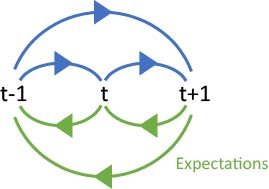
\includegraphics[width=0.3\textwidth]{Figures/ge_timing_expectations.JPG}
\end{figure}

Economic models are dynamic
\begin{itemize}
\item	They connect `yesterday' ($t-1$), `today' ($t$) and `tomorrow' ($t+1$)
\item	But so do other models (e.g. weather forecasting, bridge safety, \ldots)
\item	We share many tools with engineers, physicists\ldots	
\end{itemize}

Expectations are what make economics `special'
\begin{itemize}
\item	Our models (our world) are explicitly forward looking
\item	People make decisions with beliefs about the future in mind
\item	Aside: IoT, AI and machine learning?
\end{itemize}

\end{frame}

%%%%%%%%%%%%%%%%%%%%%%%%%%%%%%%%%%%%%%%%%%%%%%%%%%%%%%%%%%%%%%%%%%%%%%%%%%%%%
%%%%%%%%%%%%%%%%%%%%%%%%%%%%%%%%%%%%%%%%%%%%%%%%%%%%%%%%%%%%%%%%%%%%%%%%%%%%%

\begin{frame}{Macroeconomics is Stochastic}

Decision-makers must take randomness into account
\begin{itemize}
\item	Economists use the word `stochastic' to mean `randomness'
\end{itemize}
\vspace{2mm}	
We often don't know what's going to happen
\begin{itemize}
\item	We may not even know what has happened or is happening (filtering)
\end{itemize}
\vspace{2mm}
\textbf{Risk:} Even if we know how the world works there is still randomness
\begin{itemize}
\item	Playing a \textit{known} card game (don't know what's coming next but know the odds)
\end{itemize}
\vspace{2mm}
\textbf{Uncertainty:} There may also be `unknown unknowns' - \href{https://en.wikipedia.org/wiki/There_are_known_knowns}{Rumsfeld (2002)}
\begin{itemize}
\item	Like playing an \textit{unknown} card game (don't know what's coming next \textit{and} don't know the odds)
\end{itemize}

\end{frame}

%%%%%%%%%%%%%%%%%%%%%%%%%%%%%%%%%%%%%%%%%%%%%%%%%%%%%%%%%%%%%%%%%%%%%%%%%%%%%
%%%%%%%%%%%%%%%%%%%%%%%%%%%%%%%%%%%%%%%%%%%%%%%%%%%%%%%%%%%%%%%%%%%%%%%%%%%%%

\begin{frame}{Macroeconomics is Stochastic}

\begin{figure}
\centering
\label{fig:impulse_prop_fluct}
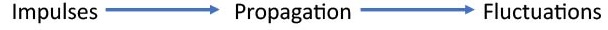
\includegraphics[width=0.5\textwidth]{Figures/impulse_prop_fluct.JPG}
\end{figure}

\textbf{Impulses:} Unexpected `structural shocks' to\ldots
	\begin{itemize}
	\item	Technology (ability to combine/reallocate resources effectively\ldots)
	\item	Monetary/fiscal policy (deviation from `standard' procedure, wars,\ldots)
	\item	Oil price, Forex and terms of trade (esp. for `small economies')
%	\item	`News' about future (forward guidance,\ldots)
	\end{itemize}
\vspace{1.5mm}
\textbf{Propagation:} How the shocks work their way through the system
	\begin{itemize}
	\item	Decisions by households and firms
	\item	Depends on preferences, technology, market structure, beliefs,\ldots
	\item	\textit{Modern} macro: explicitly microfounded and tightly parameterized
	\end{itemize}
\vspace{1.5mm}
\textbf{Fluctuations:} Due to shock propagation from current/previous periods
	\begin{itemize}
	\item	Equilibrium of a model $\Rightarrow$ probability distribution over `sequences'
	\item	Shocks and their propagation together define this distribution
	\end{itemize}

\end{frame}

%%%%%%%%%%%%%%%%%%%%%%%%%%%%%%%%%%%%%%%%%%%%%%%%%%%%%%%%%%%%%%%%%%%%%%%%%%%%%
%%%%%%%%%%%%%%%%%%%%%%%%%%%%%%%%%%%%%%%%%%%%%%%%%%%%%%%%%%%%%%%%%%%%%%%%%%%%%

\begin{frame}{Macroeconomics is General Equilibrium}

\begin{figure}
\centering
\label{fig:ge_feedback}
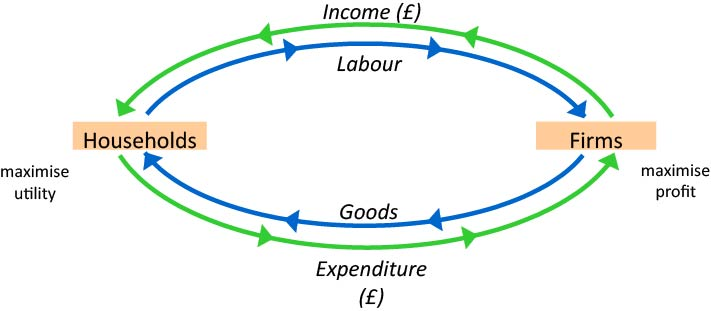
\includegraphics[width=0.3\textwidth]{Figures/ge_feedback.JPG}
\end{figure}
Markets are interconnected
	\begin{itemize}
	\item	We allow spillovers and connections between markets
	\item	Contrast with partial equilibrium (micro 101)
	\item	Typically variables are `simultaneously co-determined' in G.E.
	\end{itemize}
Simultaneity $\Rightarrow$ difficult to talk about causal relationships
	\begin{itemize}
	\item	Income depends on hours worked, depends on hiring, depends on scale of production, depends on demand, depends on income\ldots
	\end{itemize}
Interdependence of \textbf{individually optimal} decisions by multiple agents and \textbf{consistency} requirements in the aggregate
	\begin{itemize}
	\item	$\Rightarrow$ Set of simultaneous equations
	\end{itemize}

\end{frame}

%%%%%%%%%%%%%%%%%%%%%%%%%%%%%%%%%%%%%%%%%%%%%%%%%%%%%%%%%%%%%%%%%%%%%%%%%%%%%
%%%%%%%%%%%%%%%%%%%%%%%%%%%%%%%%%%%%%%%%%%%%%%%%%%%%%%%%%%%%%%%%%%%%%%%%%%%%%

\begin{frame}{Macroeconomics is General Equilibrium}

What does it mean to `solve' an economic model?
\begin{itemize}
\item	Models involve a lot of `variables' (consumption, unemployment, output, wages,\ldots)
\item	Accounting and technological constraints imply relationships among these variables
\item	The assumption that people and firms are optimizing also implies relationships among these variables
\item	There is a core set of variables that are needed to describe `the current situation' (all the relevant info.)
\item	We call these variables \textbf{`the state'}
\item	\textbf{Solving a model $\Leftrightarrow$ finding functions that relate all the variables in the economy to the state}
\end{itemize}

\end{frame}

%%%%%%%%%%%%%%%%%%%%%%%%%%%%%%%%%%%%%%%%%%%%%%%%%%%%%%%%%%%%%%%%%%%%%%%%%%%%%
%%%%%%%%%%%%%%%%%%%%%%%%%%%%%%%%%%%%%%%%%%%%%%%%%%%%%%%%%%%%%%%%%%%%%%%%%%%%%

\begin{frame}{Macroeconomics is General Equilibrium}

Remember high school math, when you had to `solve' systems of equations for $x_{1}$ and $x_{2}$
\begin{eqnarray*}
\alpha_{1,1}x_{1} + \alpha_{2,1}x_{2}	= y_{1} + z_{1}	\\
\alpha_{2,1}x_{1} + \alpha_{2,2}x_{2}	= y_{2} + z_{2}
\end{eqnarray*}
where the \textit{solution} will be $x_{1}=f_{1}(\alpha,y,z)$ and $x_{2}=f_{2}(\alpha,y,z)$

\vspace{3mm}
DSGE models' optimality conditions (Factor price ratio=MRT for firms, say) and equilibrium requirements (resource constraints, market clearing, belief consistency) will also yield a system of equations
	\begin{itemize}
	\item	More complicated (dynamics and expectations `replace' $y$ and $z$), but similar intuition
	\item	Express endogenous variables as functions of the state
	\item	The exact form of those functions will depend on the model's structure and parameters
	\end{itemize}

\end{frame}

%%%%%%%%%%%%%%%%%%%%%%%%%%%%%%%%%%%%%%%%%%%%%%%%%%%%%%%%%%%%%%%%%%%%%%%%%%%%%
%%%%%%%%%%%%%%%%%%%%%%%%%%%%%%%%%%%%%%%%%%%%%%%%%%%%%%%%%%%%%%%%%%%%%%%%%%%%%

\begin{frame}{Macroeconomics is General Equilibrium}

In practice, questions in the press are frequently poorly posed
	\begin{itemize}
	\item	\textbf{Q:} What happens to employment if inflation drops?
	\item	\textbf{A:} It depends. Is inflation falling because of looser policy or because there's been an unexpected improvement in technology?
	\end{itemize}
\vspace{2mm}
`Employment' and `inflation' are \textbf{endogenous and co-determined}
	\begin{itemize}
	\item	They may both be fluctuating because of other factors - rather than one causing the other
	\item	Causality may work in both directions via response of different agents
	\end{itemize}
\vspace{2mm}	
In micro 101 (and in a lot of old skool macro) these issues are brushed aside
	\begin{itemize}
	\item	Modern macro $\Rightarrow$ shocks are the exogenous `causal' source of fluctuations
	\item	Transmission mechanism (in equilibrium) then determines how variables co-move
	\end{itemize}

\end{frame}

%%%%%%%%%%%%%%%%%%%%%%%%%%%%%%%%%%%%%%%%%%%%%%%%%%%%%%%%%%%%%%%%%%%%%%%%%%%%%
%%%%%%%%%%%%%%%%%%%%%%%%%%%%%%%%%%%%%%%%%%%%%%%%%%%%%%%%%%%%%%%%%%%%%%%%%%%%%

\begin{frame}{DSGE models}

\begin{center}
\LARGE \textcolor{red}{D\ldots S\ldots GE}
\end{center}

Multiple periods \textcolor{red}{(D)}
	\begin{itemize}
	\item Agents form dynamic plans taking future into account
	\end{itemize}
Random shocks continually hitting the economy \textcolor{red}{(S)}
	\begin{itemize}
	\item From monetary policy and other sources (e.g. technology)
	\end{itemize}
Optimization problems of individual agents \textcolor{red}{(GE)}
	\begin{itemize}
	\item Preferences/profit maximization with budget/technological constraints
	\end{itemize}
Feasibility of optimal behavior in the aggregate \textcolor{red}{(GE)}
	\begin{itemize}
	\item Aggregation of individuals' decisions respects resource constraints
	\end{itemize}
Consistency of beliefs with the induced path of the economy \textcolor{red}{(GE)}
	\begin{itemize}
	\item Typically impose Rational Expectations requirement
	\end{itemize}

\end{frame}